\marginnote{Beginning of structure/texture.tex}

\marginnote{Retrain the grammar with EM!!!}

\begin{itemize}
\item set up some hierarchy of scales, with decompositions between them

\begin{itemize}
\item would like to use all the data we can get, which means we want
      every length of curve to be close to some scale
\end{itemize}

\item build a grammar from this
\item learn midpoint distributions by going over all pairs of curve
    points and taking the midpoint (and maybe other percentiles) by
    arclength to get triangles
\item sample from it
\item Here are samples from such a grammar, built from every class of
    the Swedish leaf dataset. Some classes are being modeled
    reasonably, some are not.
\end{itemize}


\begin{figure}
\includegraphics[width=0.45\linewidth]{experiments/7.texture/scaled_nts/output.d/scaled_nts_training_1.png}
\hfill
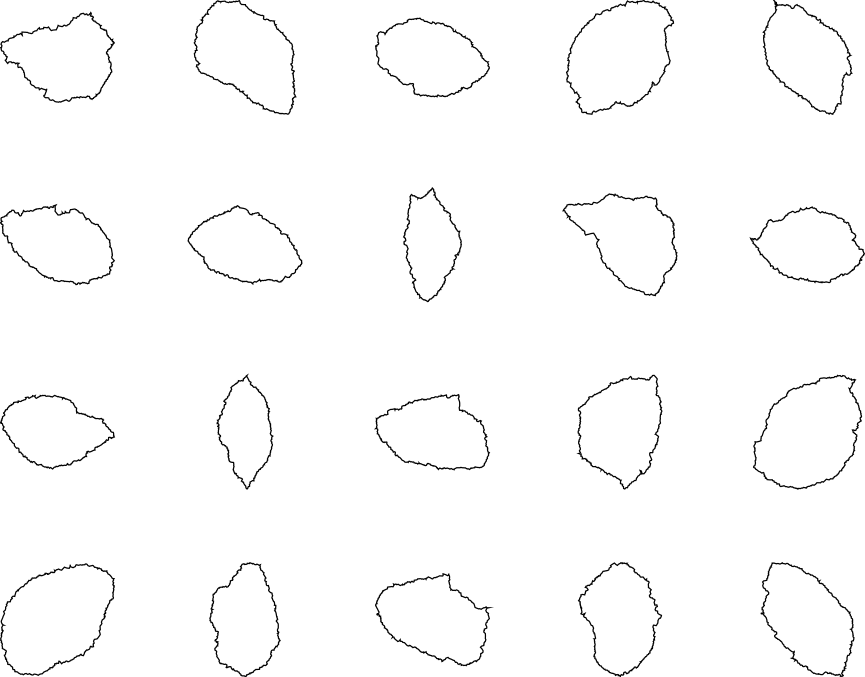
\includegraphics[width=0.45\linewidth]{experiments/7.texture/scaled_nts/output.d/scaled_nts_1.png}
\\\vspace{3\baselineskip}
\includegraphics[width=0.45\linewidth]{experiments/7.texture/scaled_nts/output.d/scaled_nts_training_2.png}
\hfill
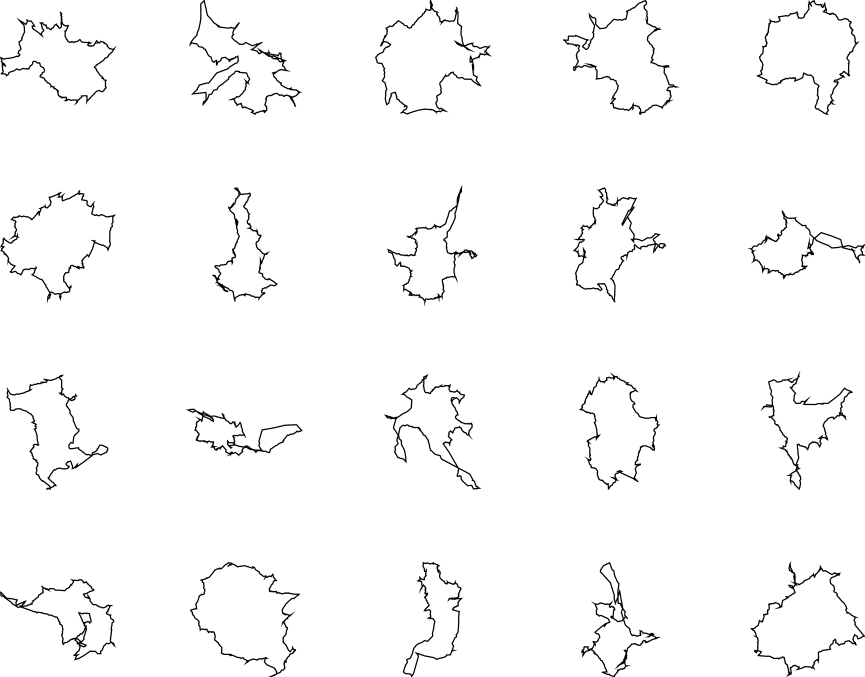
\includegraphics[width=0.45\linewidth]{experiments/7.texture/scaled_nts/output.d/scaled_nts_2.png}
\\\vspace{3\baselineskip}
\includegraphics[width=0.45\linewidth]{experiments/7.texture/scaled_nts/output.d/scaled_nts_training_3.png}
\hfill
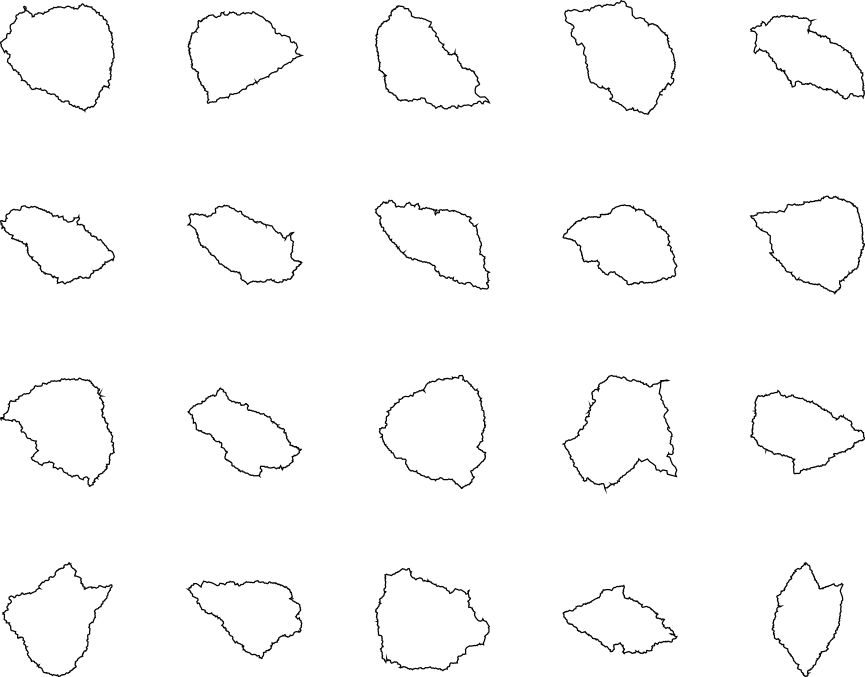
\includegraphics[width=0.45\linewidth]{experiments/7.texture/scaled_nts/output.d/scaled_nts_3.png}
\\\vspace{3\baselineskip}
\includegraphics[width=0.45\linewidth]{experiments/7.texture/scaled_nts/output.d/scaled_nts_training_4.png}
\hfill
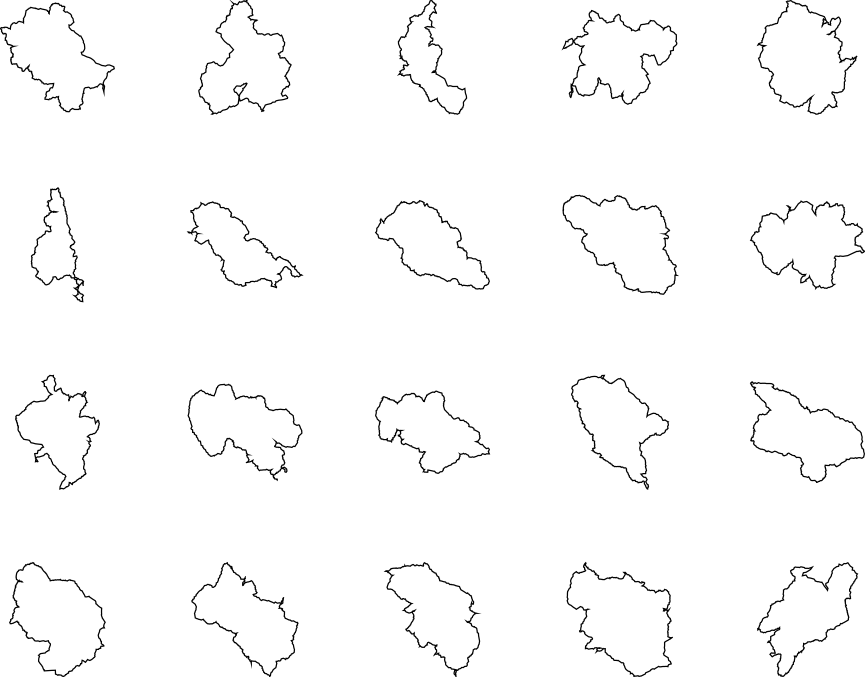
\includegraphics[width=0.45\linewidth]{experiments/7.texture/scaled_nts/output.d/scaled_nts_4.png}
\\\vspace{3\baselineskip}
\includegraphics[width=0.45\linewidth]{experiments/7.texture/scaled_nts/output.d/scaled_nts_training_5.png}
\hfill
\includegraphics[width=0.45\linewidth]{experiments/7.texture/scaled_nts/output.d/scaled_nts_5.png}
\caption{Training on left, samples on right.}
\end{figure}

\begin{figure}
\includegraphics[width=0.45\linewidth]{experiments/7.texture/scaled_nts/output.d/scaled_nts_training_6.png}
\hfill
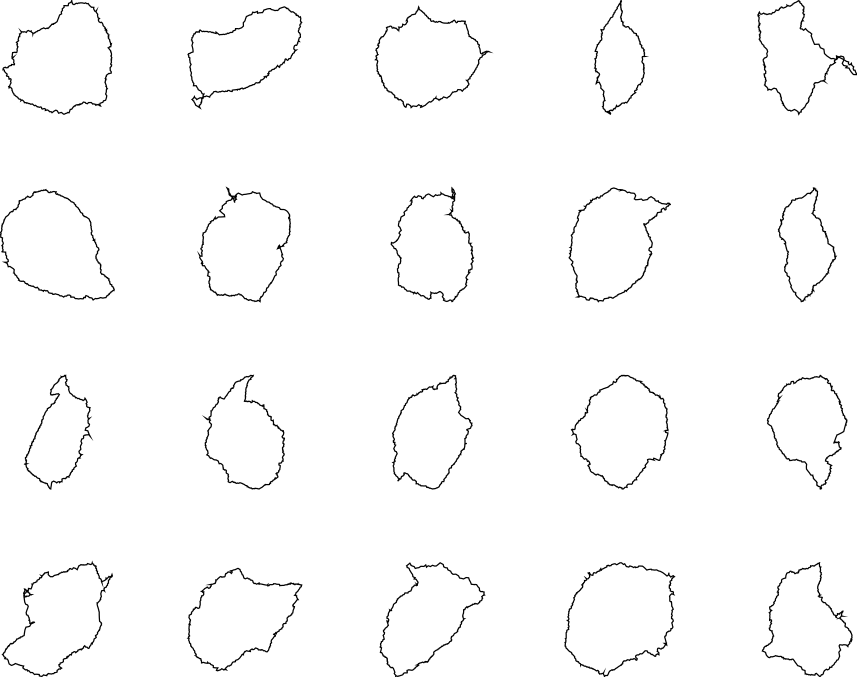
\includegraphics[width=0.45\linewidth]{experiments/7.texture/scaled_nts/output.d/scaled_nts_6.png}
\\\vspace{3\baselineskip}
\includegraphics[width=0.45\linewidth]{experiments/7.texture/scaled_nts/output.d/scaled_nts_training_7.png}
\hfill
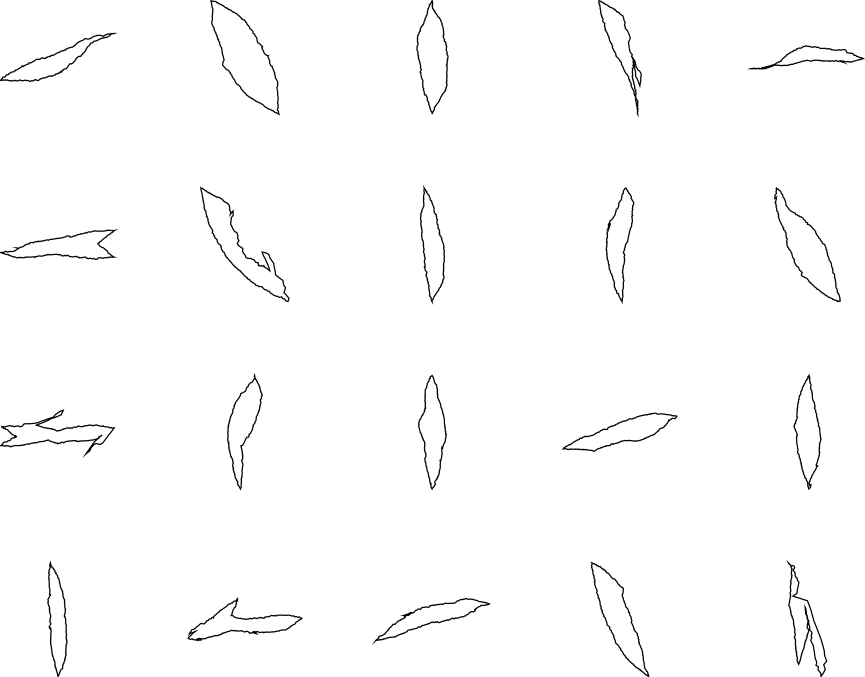
\includegraphics[width=0.45\linewidth]{experiments/7.texture/scaled_nts/output.d/scaled_nts_7.png}
\\\vspace{3\baselineskip}
\includegraphics[width=0.45\linewidth]{experiments/7.texture/scaled_nts/output.d/scaled_nts_training_8.png}
\hfill
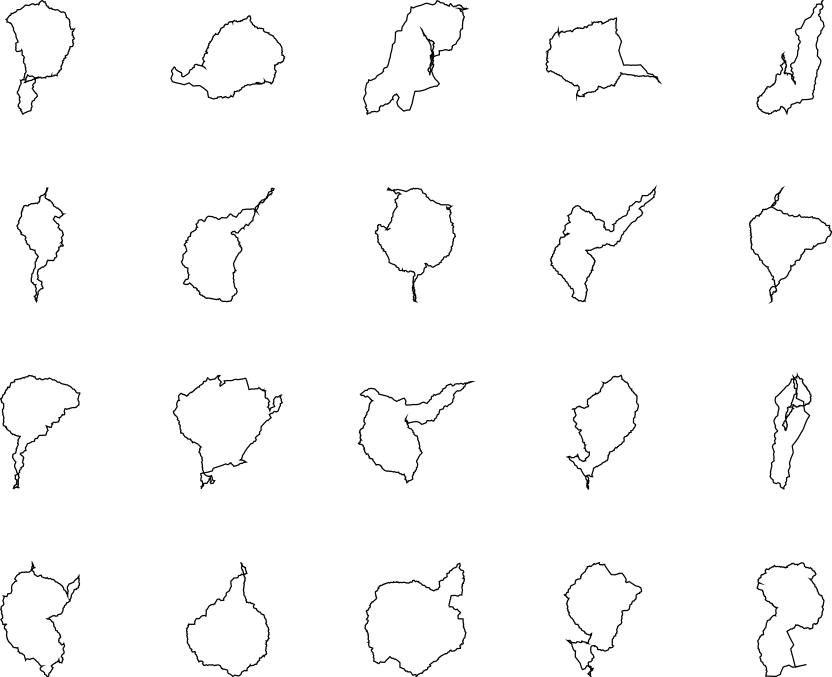
\includegraphics[width=0.45\linewidth]{experiments/7.texture/scaled_nts/output.d/scaled_nts_8.png}
\\\vspace{3\baselineskip}
\includegraphics[width=0.45\linewidth]{experiments/7.texture/scaled_nts/output.d/scaled_nts_training_9.png}
\hfill
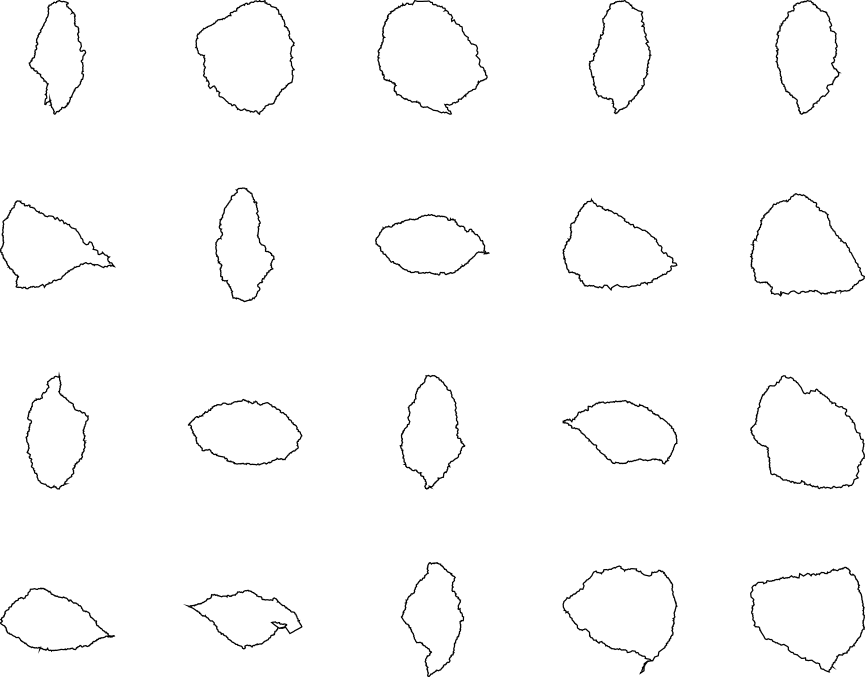
\includegraphics[width=0.45\linewidth]{experiments/7.texture/scaled_nts/output.d/scaled_nts_9.png}
\\\vspace{3\baselineskip}
\includegraphics[width=0.45\linewidth]{experiments/7.texture/scaled_nts/output.d/scaled_nts_training_10.png}
\hfill
\includegraphics[width=0.45\linewidth]{experiments/7.texture/scaled_nts/output.d/scaled_nts_10.png}
\caption{Training on left, samples on right.}
\end{figure}

\begin{figure}
\includegraphics[width=0.45\linewidth]{experiments/7.texture/scaled_nts/output.d/scaled_nts_training_11.png}
\hfill
\includegraphics[width=0.45\linewidth]{experiments/7.texture/scaled_nts/output.d/scaled_nts_11.png}
\\\vspace{3\baselineskip}
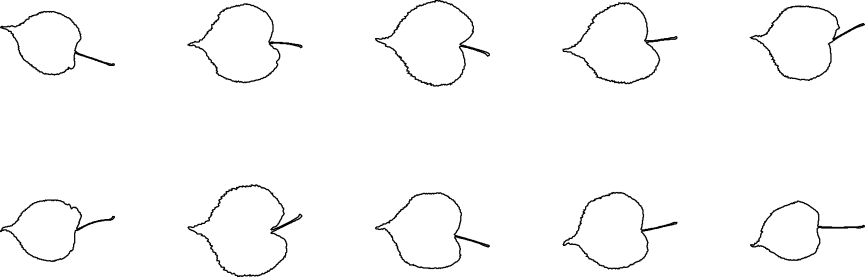
\includegraphics[width=0.45\linewidth]{experiments/7.texture/scaled_nts/output.d/scaled_nts_training_12.png}
\hfill
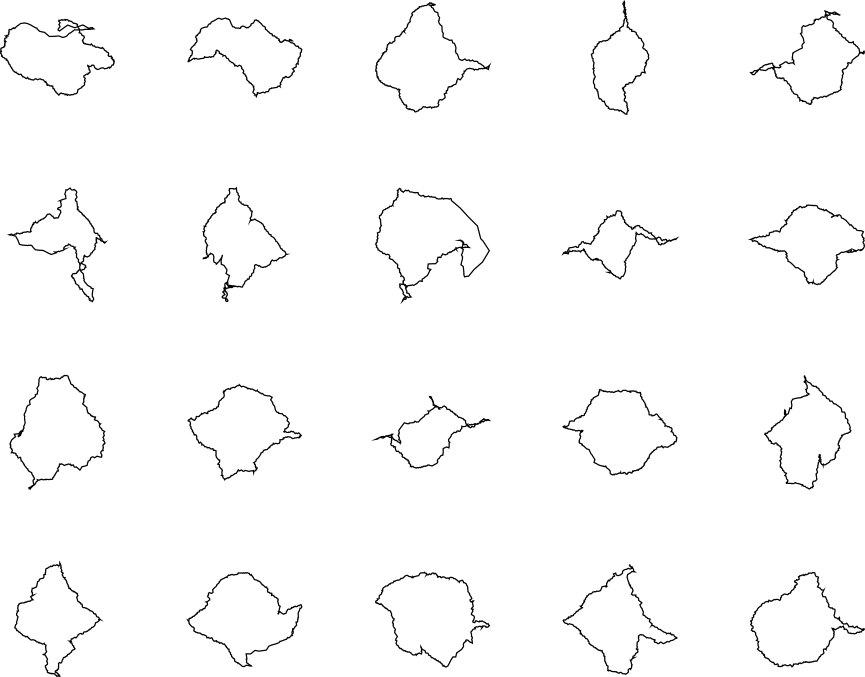
\includegraphics[width=0.45\linewidth]{experiments/7.texture/scaled_nts/output.d/scaled_nts_12.png}
\\\vspace{3\baselineskip}
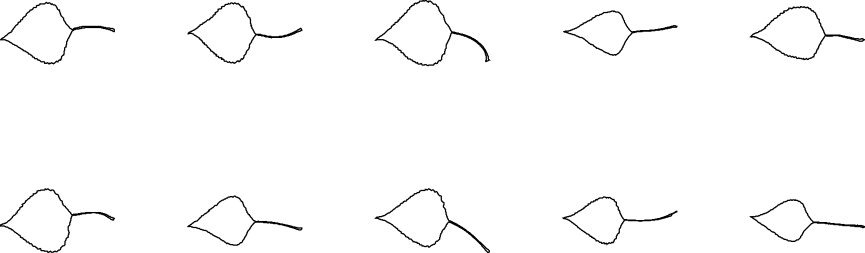
\includegraphics[width=0.45\linewidth]{experiments/7.texture/scaled_nts/output.d/scaled_nts_training_13.png}
\hfill
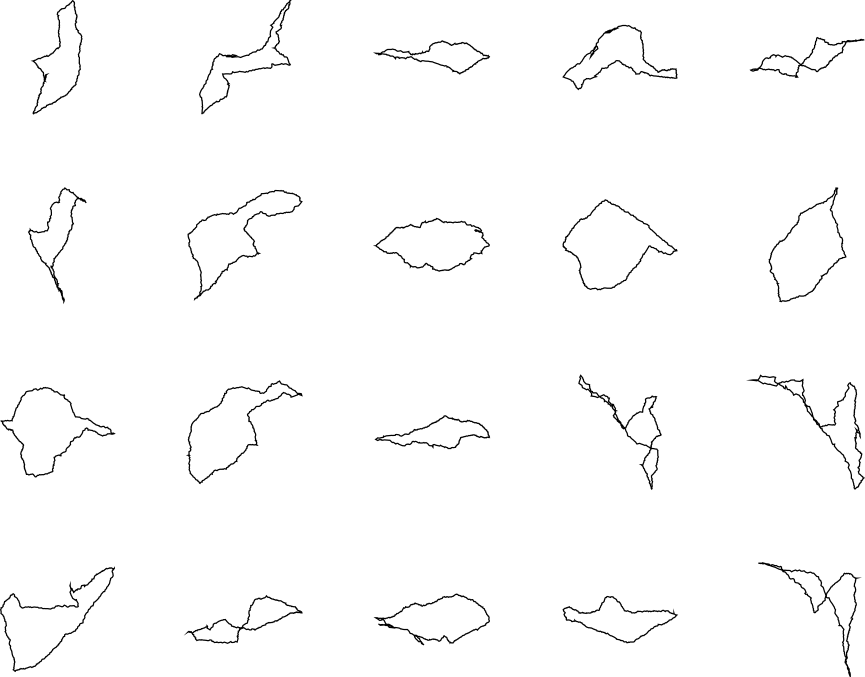
\includegraphics[width=0.45\linewidth]{experiments/7.texture/scaled_nts/output.d/scaled_nts_13.png}
\\\vspace{3\baselineskip}
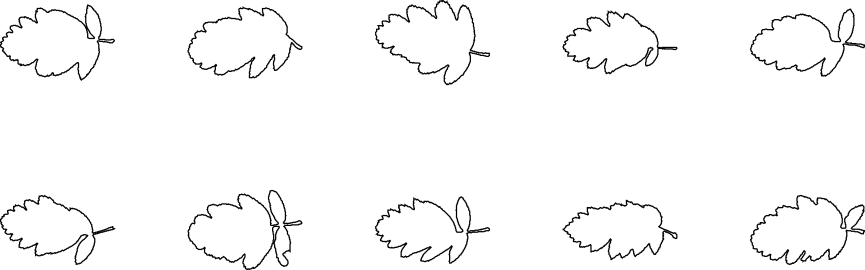
\includegraphics[width=0.45\linewidth]{experiments/7.texture/scaled_nts/output.d/scaled_nts_training_14.png}
\hfill
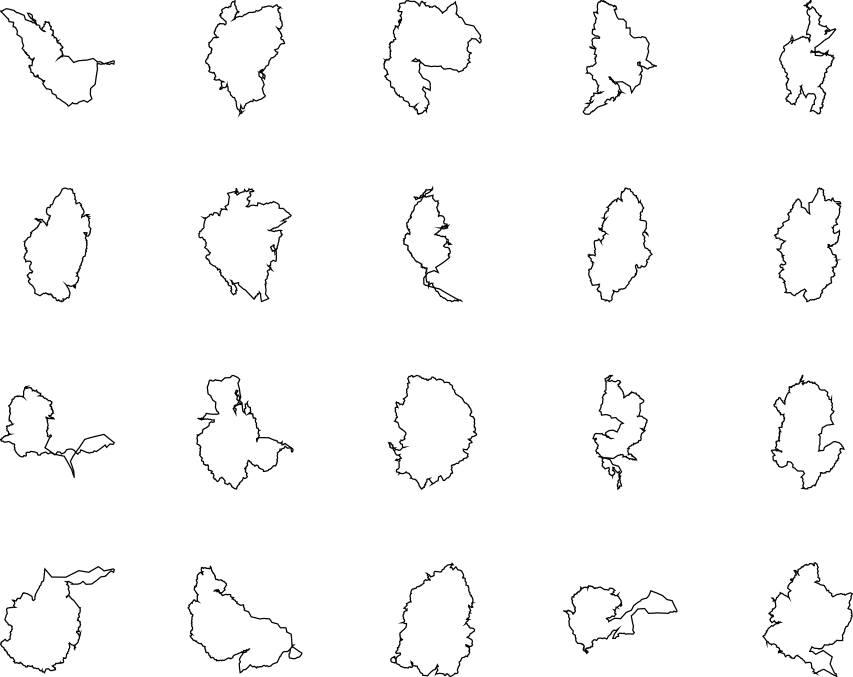
\includegraphics[width=0.45\linewidth]{experiments/7.texture/scaled_nts/output.d/scaled_nts_14.png}
\\\vspace{3\baselineskip}
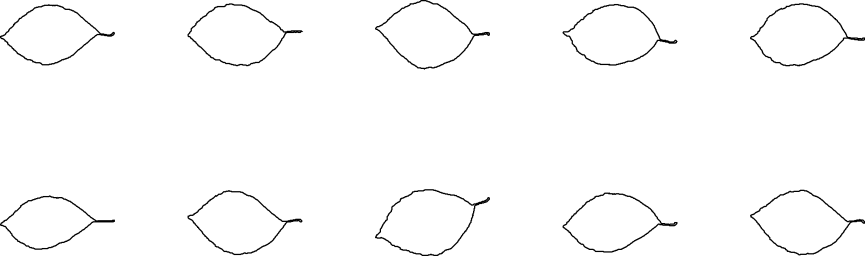
\includegraphics[width=0.45\linewidth]{experiments/7.texture/scaled_nts/output.d/scaled_nts_training_15.png}
\hfill
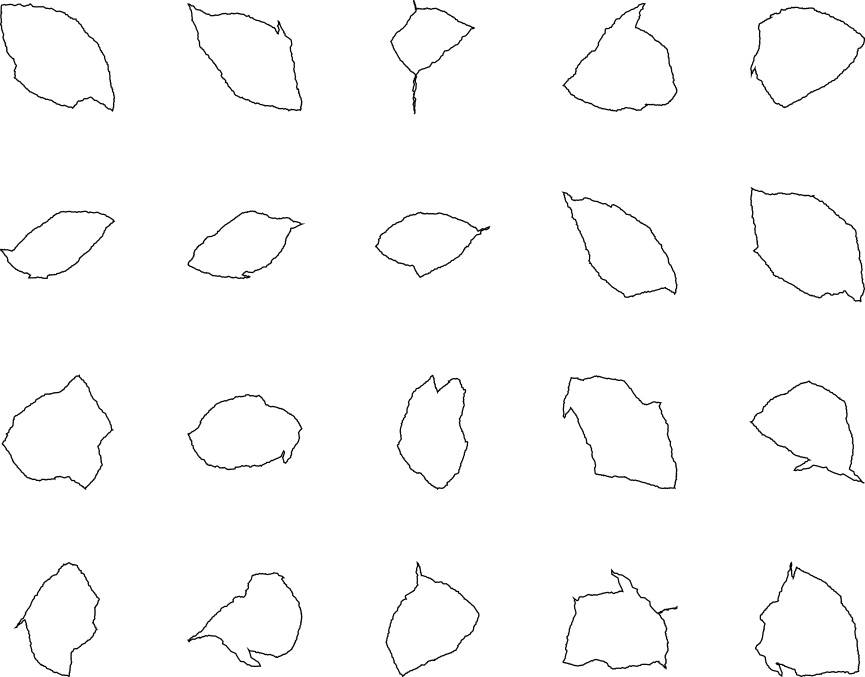
\includegraphics[width=0.45\linewidth]{experiments/7.texture/scaled_nts/output.d/scaled_nts_15.png}
\caption{Training on left, samples on right.}
\end{figure}


\marginnote{End of structure/texture.tex}
